\documentclass{standalone}
\begin{document}
		\subsection{U-Net}
		
		Artificial Neural Networks(ANN) are a computational architecture derived from neural physiological models~\cite{INP:Withey}. This architecture is made by interconnected artificial neurons able to perform elementary operations.  For imagery analysis are usually used Convolutional Neural Networks(CNN), also known as shift invariant or space invariant artificial neural networks (SIANN).\\
			
	
		In biological image processing 	the so called U-Net are usually used. U-Net is a kind of convolutional neural network which allows to overcome the requirement of many training data. That because large training dataset are not always available, like often happens in medical and biological segmentation purposes.
		
		Convolutional Networks are usually applied to classification tasks. In biological and medical purposes, the segmentation should include localization and a class label should be assigned on each voxel.
		To achieve this purposes, in $2015$ for the ISB cell tracking challenge, Olaf Ronneberger, Philipp Fischer, and Thomas Brox have developed this kind of network~\cite{ART:Johannes}.
		
		The U-Net is able to work with only small set of training samples. 	In order to work with few training data,we have to make a huge data augmentation, by applying an elastic deformation to the training images.
	
		The whole structure is divided into two main parts:
		\begin{itemize}
			\item Contraction path (\textit{encoder}) : sequence of convolutional and pooling layers, which aim
			to extract features and reduce the input dimensionality. 
			
			\item Expansion Path (\textit{decoder}) : second set of convolutional and up-sampling layers, to reconstruct the
			feature map and consequently the segmentation mask, which aims to process the extracted features
		\end{itemize}
	
		The contractive path and the extractive path. The contracting path is a typical convolutional network that consists of repeated application of convolutions, each followed by a rectified linear unit (ReLU) and a max pooling operation. During the contraction, the spatial information is reduced while feature information is increased. The expansive pathway combines the feature and spatial information through a sequence of up-convolutions and concatenations with high-resolution features from the contracting path~\cite{ART:Johannes}.
		
		Decode path tends to lose some of the higher level features that the encoder learned: Using shortcut connection, the output of the encoding layers are directly passed to the decoder layer, preserving the important features~\cite{PhDtheis}.
	
		
		\begin{figure}[h!]
			\centering
				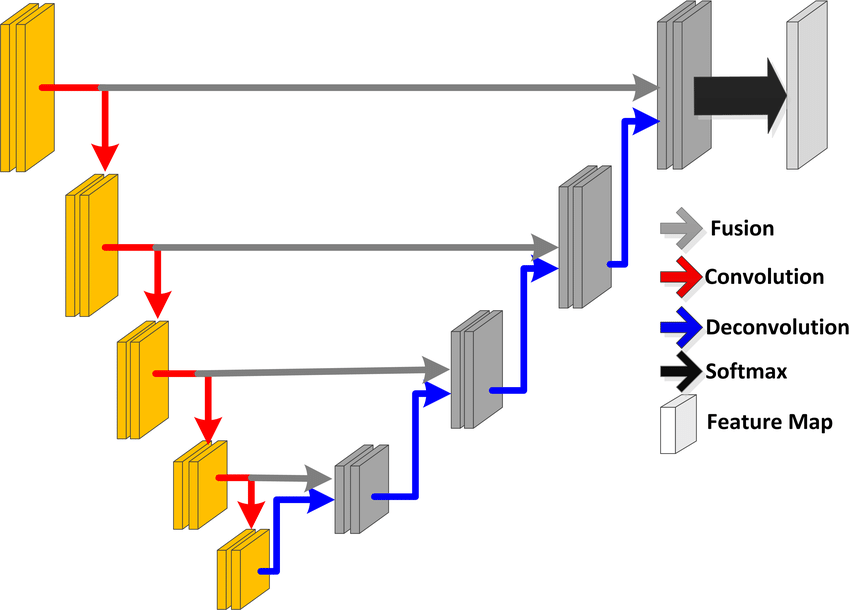
\includegraphics[scale=.4]{UNet.png}
					\caption{UNEt network architecture: We can see the U-shape made by symmetricity between expansion and contraction path. The gray arrows indicates the shortcut used to prevent information loss}\label{fig:UNet}
		\end{figure}
	
		
	
\end{document}